\documentclass[a4paper, oneside]{article}
\usepackage{graphicx} 
\usepackage{amsthm}
\usepackage{amsmath}
\usepackage{amssymb}
\usepackage[a4paper,
            bindingoffset=0.2in,
            left=2cm,
            right=2cm,
            top=2cm,
            bottom=2cm,
            footskip=.25in]{geometry}
\usepackage[italian]{babel}
\usepackage{pgfplots}
\usepackage{tabularx}
\usepackage{tikz}
\usepackage{wrapfig}
\usepackage{color}
\usepackage[d]{esvect}
\usepackage{chemfig}
\usepackage{mhchem}
\usepackage{svg}
\usepackage{float}
%\definecolor{page}{rgb}{0.129,0.157,0.212}
%\pagecolor{page}
%\color{white}
\graphicspath{ {./images/} }
\usetikzlibrary{shapes.geometric}
\usetikzlibrary{datavisualization}
\usetikzlibrary{datavisualization.formats.functions}
\usetikzlibrary{patterns}
\pgfplotsset{width=10cm,compat=1.18}

\title{Esperienza Polarizzazione}
\author{Gruppo 19 \\ Fabbri Marco, Miliani Tommaso, Mongatti Giulio, Tinacci Lorenzo}
\date{26 Novembre 2025}

\begin{document}
\newtheoremstyle{theoremEnv}
                {}          % Space above
                {}          % Space below
                {\slshape}  % Body font
                {}          % Indent amount
                {\bfseries} % Head font
                {.}         % Punctuation after head
                {\newline}  % Space after theorem head
                {}          % Theorem head spec
\theoremstyle{theoremEnv}

\newtheorem{definition}{Definizione}[section]
\newtheorem{theorem}{Teorema}[section]
\newtheorem{lemma}{Proposizione}[section]
\newtheorem{observation}{Osservazione}[section]
\newtheorem{corollary}{Corollario}[theorem]
\newtheorem{example}{Esempio}[section]
\newtheorem{remark}{Enunciato}[section]

\maketitle

\section{Scopo dell'esperienza e relazioni funzionali}
L'obiettivo dell'esperienza della polarizzazione consiste nella verifica
delle leggi di Malus. \\ Per la lamina $\frac{\lambda}{2}$:
\begin{align}
    I_\parallel(\theta) &= I_0 \cos^{2}(2\theta) \\
    I_\perp(\theta) &= I_0 \sin^{2}(2\theta)
\end{align}
Mentre per la lamina $\frac{\lambda}{4}$: 
\begin{align}
    I_\parallel &= I_0\left(1 - \frac{1}{2}\sin^{2}(2\theta)\right) \\
    I_\perp &= \frac{I_0}{2}\sin^{2}(2\theta).
\end{align}
Dove si definiscono i seguenti elementi:
\begin{itemize}
    \item $\theta$: angolo di rotazione dell’asse fast e l’asse slow di ciascuna lamina di ritardo
     attorno ad un asse parallelo alla direzione di propagazione dell’onda elettromagnetica entrante.
     Si sceglie per convenzione 0° come l’angolo per cui i suddetti assi coincidono con le direzioni
     delle due componenti lungo cui si scompone il campo elettrico (una parallela, l’altra ortogonale 
     rispetto al piano di incidenza dell’onda).
    \item $I_0$: intensità dell’onda precedentemente all’entrata di essa nella lamina di ritardo con
    campo elettrico dato dalla sola componente parallela al piano di incidenza.
\end{itemize}
Inoltre ci proponiamo di mostrare qualitativamente il diverso comportamento
delle due lamine in seguito ad un doppio passaggio di un fascio di luce. \\ \\
Per la validità della verifica sperimentale, si ipotizza che:
\begin{itemize}
    \item il laser utilizzato abbia una potenza costante nel tempo.
    \item L’onda elettromagnetica uscente dal laser sia idealmente piana e che incida
    sul film dielettrico dei cubi polarizzatori con un angolo di incidenza di $\frac{\pi}{4}$ rispetto
    alla normale del film birifrangente.
    \item Le facce dei cubi polarizzatori e delle lamine siano perfettamente ortogonali alla direzione di propagazione dell’onda.
    \item Che il cubo polarizzatore sia di fattura ideale:
    \begin{gather*}
        n_\perp = n_{\text{vetro}} \frac{\sqrt{2} }{2} \qquad n_\parallel = n_{\text{vetro}} 
    \end{gather*}
\end{itemize}
Dove con $n_\perp$ e $n_\parallel$ si indicano gli indici di rifrazione.
\clearpage

\section{Schema generale di misura}
L’esperienza consiste nel preparare un fascio laser, di potenza costante, con una polarizzazione
lineare mediante un cubo polarizzatore detto di pulizia. Successivamente il fascio attraversa 
una lamina con asse slow inclinato di un angolo $\theta$ rispetto alla direzione iniziale della polarizzazione.
Sfruttando un secondo cubo, detto di analisi, è possibile misurare la potenza trasmessa e riflessa al variare di $\theta$. 
Le 20 misure sono analizzate mediante un programma scritto in Mathematica. Effettuando un fit non-lineare mediante la funzione 
\begin{align}
    f(a, b, \phi, o, x) = a\cos^{2}(bx + \phi) + o
\end{align}
è possibile verificare se le curve che meglio descrivono l’andamento dei dati sperimentali corrispondono,
entro le barre di errore associate ai parametri liberi del fit, alle equazioni delle leggi di Malus.
In caso affermativo si considerano verificate le suddette leggi.

\section{Apparato Sperimentale}
\begin{gather*}
    \begin{tikzpicture}[scale=1.2]
        \filldraw[cyan](-1, 0) circle (0.1) node[anchor = north] {\tiny sorgente};
        \draw(-0.25, 0) circle (0.1);
        \filldraw(0.5, 0) circle (1pt);
        \draw[->](-0.25, -0.1) -- (-0.25, -1) node[at end, right] {$\hat{z} $};
        \filldraw(-0.25, 0) circle (1pt) node[anchor = south] {$\hat{y} $};
        \draw(0.5, 0) circle (0.1) node[anchor = north] {$\vv{E_{0y}} $};
        \draw(0.5, 0) circle (1pt);
        \draw[->](0.5, 0.1) -- (0.5, 1) node[at end, right] {$\vv{E_{0z}}$};
        \draw[pattern = north west lines, pattern color = white](1.25, -0.5) rectangle (1.75, 0.5);
        \node[align = center] at (1.5, 0.8) {\tiny filtro};
        \node at (1.5, 0.65) {\tiny intensità};
        \draw (2.5, -0.5) rectangle (3.5, 0.5);
        \draw(2.5, 0.5) -- (3.5, -0.5);
        \node at (3, 0.6) {\tiny cubo pulizia};
        \draw[->](4.5, 0) -- (4.5, 1) node[at end, right] {$\vv{E_{0z}}$};
        \draw(5.5, -0.5) rectangle (6, 0.5);
        \node[align = center] at (5.75, 0.6) {\tiny lamina di ritardo};
        \draw[->](7, 0.1) -- (7, 0.5) node[at end, right] {$\vv{E_{0z}}$};
        \filldraw(7, 0) circle (1pt) node[anchor = north] {$\vv{E_y}$};
        \draw(7, 0) circle (0.1);
        \draw(8, -0.5) rectangle (9, 0.5);
        \node at (8.5, 0.6) {\tiny cubo analisi};
        \draw(8, 0.5) -- (9, -0.5);
        \draw(8.5, -1) circle (0.1) node[anchor = west] {$\vv{E_{0y}} $};
        \filldraw(8.5, -1) circle (1pt);
        \draw[->](8.5, 0) -- (9.25, 0);
        \draw[->](9.5, 0) -- (9.5, 0.5) node[at end, right] {$\vv{E_z}$}; 
        \draw(8, -1.5) rectangle (9, -2);
        \node at (8.5, -1.75) {\tiny rilevatore};
        \draw[dashed](8.5, -1.5) -- (8.5, 0);
        \draw[dashed](-0.75, 0) -- (10, 0);
        \draw(10, -0.25) rectangle (11, 0.25) node[midway] {\tiny rilevatore};
    \end{tikzpicture}
\end{gather*}
La sorgente luminosa è un laser a diodo in continua alla lunghezza d’onda di $\lambda = 532 \ nm$.
I rilevatori utilizzati sono due fotodiodi al silicio il cui segnale può essere misurato
mediante due multimetri. Tali rilevatori hanno una risposta pressoché lineare in un
intervallo di circa 10 Volt, per cui viene posto davanti alla sorgente un filtro
regolabile per assicurarsi di non superare tale valore. Davanti ai rilevatori sono
posti dei filtri ulteriori in modo tale che venga filtrata la luce della stanza e
che possa passare solamente la luce con lunghezza d’onda vicino a 532 nm.
Per effettuare la calibrazione dei due rilevatori, si ricorre alla lamina $\frac{\lambda}{2}$ che ci
permette di inviare una potenza luminosa ben definita (perché costante in un breve
intervallo di tempo) prima su un rilevatore e subito dopo sull'altro. Per cui, per ogni rilevatore, 
si sono ricavati, ruotando la lamina, i valori massimi. Per ciascuno di questi due valori, si sono
successivamente normalizzate le intensità misurate dal corrispondente rilevatore da cui è stato letto.
Alle varie misure è sottratto un offset ottenuto dalla lettura del valore indicato da ciascun rilevatore in
azione in assenza del raggio laser incidente. La misura non viene effettuata
tappando i rilevatori, ma bloccando unicamente l’uscita del laser, in maniera tale da
considerare nell’offset l’intensità rilevata della luce della stanza non bloccata dal filtro (che può comunque,
di per sé, essere soggetta a fluttuazioni). Come si legge dai dati, la differenza degli offset misurati per
ciascun rilevatore rientra nell’errore di sensibilità. Ogni lamina è inserita all’interno di un rotatore goniometrico. \\ 
Le incertezze associate agli strumenti utilizzati sono le seguenti:
\begin{itemize}
    \item Multimetri: $0.01$ Volt.
    \item Rotatore goniometrico delle lamine: $2^{\circ}$;
    \item Offset rilevatore: $0.03$ Volt e $0.04$ Volt. 
\end{itemize}
Dopo aver opportunamente regolato il filtro, per quanto riguarda l'intensità 
massima dei due fasci, abbiamo ottenuto i seguenti valori: 
\begin{itemize}
    \item Fascio riflesso: $8.96$ Volt;
    \item Fascio trasmesso: $9.67$ Volt. 
\end{itemize}
Si sono dunque utilizzati questi valori come coefficienti di calibrazione
per poter ottenere fit sinusoidali comparabili. Di seguito vi è una schematizzazione
dell'apparato sperimentale utilizzato per la doppia riflessione:
\begin{gather*}
    \begin{tikzpicture}
        \draw[dashed](0.5, 0) -- (8, 0);
        \draw(-1.5, -0.4) rectangle (0.5, 0.4);
        \draw[thick](8, -1) -- (8, 1);
        \node at (2.1, 0.75) {filtro};
        \filldraw[pattern= north west lines] (8, 1) rectangle (8.25, -1);
        \draw(2, 0.5) rectangle (2.25, -0.5);
        \draw(3, 0.5) rectangle (4, -0.5);
        \draw(3, 0.5) -- (4, -0.5);
        \draw(3.5, 0) -- (3.5, -1.5);
        \draw(3.25, -1.5) rectangle (3.75, -2.5);
        \node at (2.3, -2) {rilevatore};
        \node at (8.15, 1.2) {specchio};
        \draw(5.75, 0.5) rectangle (6.25, -0.5);
        \node at (6, 0.75) {lamina}; 
        \node at (-0.5, 0) {laser};
    \end{tikzpicture}
\end{gather*}

\section{Misure e analisi}
\subsection{Lamina $\frac{\lambda}{2}$}
Qui di seguito si riporta una tabella delle intensità dove, ad ogni angolo del rotatore goniometrico,
corrisponde una potenza misurata per il rilevatore della luce riflessa e quella trasmessa.
\begin{gather*}
    \begin{tabular}{ c  c  c }
        \hline
        Angolo Misura & Potenza misurata(Volt) $\perp$ & Potenza misurata(Volt) $\parallel$ \\
        \hline
        0° & 0.30  & 9.23  \\
        18° & 4.64 & 4.65 \\
        36° & 8.84 & 0.21 \\
        54° & 7.12 & 2.18 \\
        72° & 1.79 & 7.97 \\
        90° & 0.32 & 9.49 \\
        108° & 4.79 & 4.72 \\
        126° & 9.01 & 0.22 \\
        144° & 7.19 & 2.21 \\
        162° & 1.70 & 8.05 \\
        180° & 0.38 & 9.46 \\
        198° & 5.00 & 4.49 \\
        216° & 9.09 & 0.14 \\
        234° & 7.00 & 2.45 \\
        252° & 1.63 & 8.21 \\
        270° & 0.37 & 9.58 \\
        288° & 4.92 & 4.76 \\
        306° & 9.16 & 0.20 \\
        324° & 7.30 & 2.23 \\
        342° & 1.84 & 8.09 \\
        \hline
    \end{tabular}
\end{gather*}
Dato che le due potenze massime distano di ben 0.71 Volt, la discrepanza  non è comparabile con l'errore
di sensibilità dello strumento ed è da attribuirsi al fatto che i due rilevatori utilizzati,
nonostante siano lo stesso modello, possano rispondere in maniera diversa
a sollecitazioni uguali. 
Da queste misure si è ottenuto, tramite il programma scritto in Mathematica, il seguente
fit sinusoidale:
    \begin{figure}[H]
        \centering
        \includesvg[width=0.6\textwidth]{grafico_funzioni-Lambda_mezzi.svg}
    \end{figure}
Il fit restituisce i seguenti dati sperimentali 
per le due curve dell'intensità dell'onda riflessa sul cubo di analisi:
\begin{itemize}
    \item $a \pm \Delta a = 1.022 \pm 0.008$;
    \item $b \pm \Delta b = 2.003 \pm 0.002$;
    \item $\phi \pm \Delta \phi = 1.742 \pm 0.007$;
    \item $o \pm \Delta o = 0.002 \pm 0.005$.  
\end{itemize}
Mentre per quanto riguarda il fit sinusoidale dell'onda trasmessa 
restituisce i seguenti dati:
\begin{itemize}
    \item $a \pm \Delta a = 1.012\pm 0.007$;
    \item $b \pm \Delta b = 2.001\pm 0.002$;
    \item $\phi \pm \Delta \phi = 0.185\pm 0.007$;
    \item $o \pm \Delta o = -0.001\pm 0.005$. 
\end{itemize}
\paragraph{Analisi quantitativa sui parametri del fit}\mbox{}\\
Dai valori calcolati dal fit, si osserva che i valori di $a$ distano tra di loro di $\sim 0.7\sigma$, dove
$\sigma = \sigma_a^{\parallel} + \sigma_a^{\perp}$. Si noti inoltre che entrambe
le misure di $a$ risultano essere più lontane dal valore atteso $a = 1$ (rispettivamente di
$\sim 2.7\sigma_a^{\perp}$ e di $\sim 1.7\sigma_a^{\parallel}$ per il fascio 
riflesso e trasmesso). Dato che le ampiezze dei fit risultano compatibili tra di loro,
si è ipotizzato che il discostamento significativo dei valori di $a$ misurati rispetto al
valore teorico sia dovuto alla variazione di intensità del laser col tempo. Si riporta nel seguente grafico 
l'intensità totale misurata dai rilevatori in funzione delle nostre misure.
\begin{figure}[H]
    \centering
    \includesvg[width=0.6\textwidth]{intensità_totale-Lambda_mezzi.svg}
\end{figure} 
Per quanto riguarda le fasi, la loro differenza $\phi_\perp - \phi_\parallel$ è di 
$\phi_D = 1.557 \pm 0.014$, che è compatibile col valore atteso di $\overline{\phi_D} = 1.5710$ (infatti la differenza di fasi si discosta
di un $\sigma_\phi$).  
Per quanto riguarda il coefficiente $b$,
ottenuto dal programma di fit, si osserva che il suo valore, nel caso della luce riflessa dal cubo, 
dista dal valore atteso di $1.5 \sigma_b$, mentre, per quanto riguarda la luce trasmessa, il suo valore è
entro un $\sigma_b$. Infine, la distanza per i valori degli offset
risulta essere di $0.4\sigma_o$ e $0.2\sigma_o$ rispettivamente per il fascio
riflesso e quello trasmesso. 

\paragraph{Possibili correzioni sulla fase e sulla pulsazione}\mbox{}\\
Nonostante i valori di $b$ siano compatibili con il valore atteso ($ \overline{b} = 2$ ), si è fatta ipotesi che,
data l'alta incertezza associata al rotatore goniometrico, sia stato compiuto qualche errore di lettura
sull'angolo che non ci ha permesso di ottenere valori ancora più vicini a quelli attesi. Per verificare ciò, abbiamo scelto di variare di un grado (198° a 199°) 
l’angolo relativo ad un valore sensibile, ovvero un valore di intensità lontano dai massimi e dai 
minimi teorici (dove la derivata è massima). Si è ottenuto dunque un valore di $b$
sensibilmente più preciso: per il fascio riflesso la distanza è diminuita a un $\sigma_b$ dal valore atteso, mentre per
quanto riguarda il fascio trasmesso rientra comunque dentro un $\sigma_b$. 
La differenza di fasi, invece, è aumentata leggermente a $\phi_D = 1.558 \pm 0.014$, mentre l'errore assoluto è
diminuito leggermente a $\sim 0.8\sigma_\phi$. Infine, anche la distanza dal valore 
atteso degli offset è ulteriormente diminuita: per il fascio riflesso il valore dell'offset
è diventato direttamente comparabile con il valore teorico, mentre l'offset per il 
fascio trasmesso è rimasto distante di $0.2\sigma_o$ rispetto al valore atteso. Si riportano 
dunque i dati trovati per i due fit:
\begin{itemize}
    \item $a \pm \Delta a = 1.021 \pm 0.008$;
    \item $b \pm \Delta b = 2.002 \pm 0.002$;
    \item $\phi \pm \Delta \phi = 1.741 \pm 0.007$;
    \item $o \pm \Delta o = 0.000 \pm 0.005$.  
\end{itemize}
Mentre per il fit trasmesso:
\begin{itemize}
    \item $a \pm \Delta a = 1.011\pm 0.008$;
    \item $b \pm \Delta b = 2.000 \pm 0.002$;
    \item $\phi \pm \Delta \phi = 0.183 \pm 0.007$;
    \item $o \pm \Delta o = 0.001 \pm 0.005$. 
\end{itemize}
\begin{figure}[H]
    \centering
    \includegraphics[width=0.65\textwidth]{lambda-mezzi-correzione.pdf}
\end{figure} 



\subsection{Lamina $\frac{\lambda}{4}$}
Qui di seguito riportiamo i grafici e le tabelle delle potenze misurate al variare
dell’angolo del rotatore contenente la lamina $\frac{\lambda}{4}$ e i 
risultati del fit non lineare. Nella tabella, ad ogni angolo del rotatore goniometrico,
corrisponde una potenza misurata per il rilevatore della luce riflessa e quella trasmessa.
\begin{gather*}
    \begin{tabular}{ c  c  c }
        \hline
        Angolo Misura & Potenza misurata (Volt) $\perp$ & Potenza misurata (Volt) $\parallel$ \\
        \hline
        0° & 2.41 & 6.90  \\
        18° & 4.30 & 4.79 \\
        36° & 3.25 & 5.97 \\
        54° & 0.74 & 8.63 \\
        72° & 0.23 & 9.09 \\
        90° & 2.38 & 6.74 \\
        108° & 4.34 & 4.77 \\
        126° & 3.39 & 5.94 \\
        144° & 0.84 & 8.80 \\
        162° & 0.19 & 9.49 \\
        180° & 2.37 & 7.08 \\
        198° & 4.27 & 4.88 \\
        216° & 3.30 & 6.05 \\
        234° & 0.78 & 8.88 \\
        252° & 0.22 & 9.56\\
        270° & 2.50 & 7.01\\
        288° & 4.50 & 4.79 \\
        306° & 3.55 & 5.86 \\
        324° & 0.88 & 8.71 \\
        342° & 0.20 & 9.36 \\
        \hline
    \end{tabular}
\end{gather*}
Anche per questo gruppo di misurazioni si sono utilizzate le potenze massime,
come si è precedentemente fatto per la prima lamina, come coefficienti di calibrazione. 
Da queste misure si è ottenuto, tramite il programma scritto in Mathematica, il seguente
fit sinusoidale.
\begin{figure}[H]
    \centering
    \includegraphics[width=0.6\textwidth]{lambda-quarti.pdf}
\end{figure} 
Il fit sinusoidale calcolato restituisce i seguenti dati sperimentali 
per le due curve dell'intensità dell'onda riflessa sul cubo di analisi:
\begin{itemize}
    \item $a \pm \Delta a = 0.488 \pm 0.006$;
    \item $b \pm \Delta b = 1.996 \pm 0.003$;
    \item $\phi \pm \Delta \phi = -0.735 \pm 0.011$;
    \item $o \pm \Delta o = 0.001 \pm 0.003$.  
\end{itemize}
Mentre per quanto riguarda il fit sinusoidale dell'onda trasmessa 
restituisce i seguenti dati:
\begin{itemize}
    \item $a \pm \Delta a = 0.498\pm 0.008$;
    \item $b \pm \Delta b = 1.995 \pm 0.004$;
    \item $\phi \pm \Delta \phi = 0.849\pm 0.015$;
    \item $o \pm \Delta o = 0.489 \pm 0.005$. 
\end{itemize}
\paragraph{Analisi quantitativa delle misure}\mbox{}\\
I valori ottenuti dal fit per il parametro $a$ distano tra di loro di $\sim 0.8\sigma$, dove
$\sigma = \sigma_a^{\parallel} + \sigma_a^{\perp}$. Tali valori risultano, inoltre, confrontandoli con quelli 
della $\frac{\lambda}{2}$, più vicini al valore atteso $\overline{a} = 1$: $a_\perp$ si discosta di $\sim 2\sigma_a$, mentre
$a_\parallel$ rientra di gran lunga entro il limite del singolo sigma ($\sim0.3\sigma_a$).
Supponiamo che, fatta pratica con le precedenti misure, ciò sia dovuto ad una presa dati più rapida da parte di noi sperimentatori,
per cui il laser non ha avuto modo di aumentare sensibilmente la sua intensità, risultando dunque in parametri migliori del fit.
Tuttavia, ciò non ha portato ad una miglior compatibilità tra le due misure di $a$.
Anche per le stime di $b$ abbiamo ottenuto valori inferiori al valore atteso $\overline{b} = 2$, 
discostandosi di $\sim1.3\sigma_b$ per $b_\perp$ e di $\sim1.3\sigma_b$ per $b_\parallel$.
La differenza tra le fasi $\phi_\parallel$ e $\phi_\perp$ rientra nei valori attesi:
$\phi_D = 1.58 \pm 0.03$. Per quanto riguarda gli offset, uno di loro è più vicino al
valore atteso di $\overline{o} = 0.5$: l'offset del fascio di luce trasmesso ha un
discostamento di $\sim0.3\sigma_o$ mentre per quanto riguarda il fascio riflesso
ha un discostamento di $\sim 2.2\sigma_o$.
\begin{figure}[H]
    \centering
    \includesvg[width=0.55\textwidth]{intensità_totale-Lambda_quarti.svg}
\end{figure} 
\paragraph{Possibili correzioni applicabili al fit}\mbox{}\\
Visti i dati del fit sinusoidale, si è provato a modificare leggermente gli angoli 
delle misure ottenute, così come si è fatto per la lamina $\frac{\lambda}{2}$, 
ma non si è osservato nessun miglioramento significativo per i dati dei due fit. 


\subsection{Retroriflessione}
\paragraph{Dati della retroriflessione per le due lamine}
\begin{gather*}
    \text{Retroriflessione lamina } \frac{\lambda}{4} \qquad \qquad \qquad \qquad \qquad \text{Retroriflessione lamina } \frac{\lambda}{2}\\
    \begin{tabular}{ c  c }
        \hline
        Angolo Misura & Potenza misurata (Volt) \\
        \hline
        0° & 5.03 \\
        18° & 8.95 \\
        36° & 6.83\\
        54° & 1.53 \\
        72° & 0.42 \\
        90° & 5.06  \\
        108° & 9.35  \\
        126° & 7.23  \\
        144° & 1.69 \\
        162° & 0.39\\
        180° & 5.17  \\
        198° & 9.44  \\
        216° & 7.07 \\
        234° & 1.55  \\
        252° & 0.42 \\
        270° & 5.99\\
        288° & 9.99  \\
        306° & 7.56 \\
        324° & 1.76 \\
        342° & 0.41  \\
        \hline
    \end{tabular}
    \qquad 
     \begin{tabular}{ c  c }
        \hline
        Angolo Misura & Potenza misurata (Volt) \\
        \hline
        0° & 0.05 \\
        18° & 0.03 \\
        36° & 0.03\\
        54° & 0.03 \\
        72° & 0.02 \\
        90° & 0.02  \\
        108° & 0.03  \\
        126° & 0.04  \\
        144° & 0.05  \\
        162° & 0.05 \\
        180° & 0.05  \\
        198° & 0.03  \\
        216° & 0.03  \\
        234° & 0.03  \\
        252° & 0.03 \\
        270° & 0.02 \\
        288° & 0.03  \\
        306° & 0.05  \\
        324° & 0.07 \\
        342° & 0.08  \\
        \hline
    \end{tabular}
\end{gather*}

\clearpage
\paragraph{Analisi dati retroriflessione}\mbox{}\\
Da questi dati si è ottenuto  il seguente grafico per le due lamine
\begin{figure}[H]
    \centering
    \includegraphics[width=0.55\textwidth]{fit-riflessione-non-normalizzata.pdf}
\end{figure} 
Per la retroriflessione della lamina $\frac{\lambda}{4}$ si è ottenuto i seguenti dati del fit
sinusoidale: 
\begin{itemize}
    \item $a \pm \Delta a = 9.53 \pm 0.19$;
    \item $b \pm \Delta b = 2.003 \pm 0.006$;
    \item $\phi \pm \Delta \phi = 2.40 \pm 0.02$;
    \item $o \pm \Delta o = 0.00 \pm 0.12$.  
\end{itemize}
Mentre per quanto riguarda la lamina $\frac{\lambda}{2}$ si hanno i seguenti dati:
\begin{itemize}
    \item $a \pm \Delta a = -0.017\pm 0.011$;
    \item $b \pm \Delta b = 2.067 \pm 0.162$;
    \item $\phi \pm \Delta \phi = -0.9 \pm 0.6$;
    \item $o \pm \Delta o = 0.02 \pm 0.01$. 
\end{itemize}
I valori di $a$ per i due fit differiscono dal valore atteso di $\overline{a} = 1$ di ben $\sim 2.5\sigma_a$ per
la $\frac{\lambda}{4}$ e di $\sim 1.5\sigma_a$ per la $\frac{\lambda}{2}$.  
Sospettiamo che la variazione continua dell’intensità del laser 
abbia introdotto anche su queste misure un errore sistematico. Inoltre è probabile che il cubo 
non fosse allineato perfettamente con l’asse ottico del sistema, provocando 
una piccola differenza tra l’angolo di incidenza di partenza e quello di ritorno. 
Rispetto al valore di $\overline{b}= 2$, il valore trovato di $b$ per la $\frac{\lambda}{4}$ 
differisce di $\sim0.5\sigma_b$, mentre per il fit sinusoidale della $\frac{\lambda}{2}$ differisce $\sim 0.4\sigma_b$.
Si vede dunque che la deriva dell’intensità del laser non ha influenzato in modo 
significativo le misure di $b$, che risultano compatibili tra di loro. Infine, nel caso del doppio attraversamento della 
lamina $\frac{\lambda}{4}$, l'offset risulta comparabile con il valore atteso dell'offset
del fit, mentre per il doppio attraversamento della $\frac{\lambda}{2}$ risulta
essere più distante a $\sim 2\sigma_o$ rispetto al valore atteso.
La differenza di fase $\phi_D$ invece risulta essere distante di $\sim0.1\sigma_\phi$
dal valore atteso $\overline{\phi_D} = 1.571$.   
\begin{figure}[H]
    \centering
    \includesvg[width=0.6\textwidth]{intensità_totale_Riflessione.svg}
\end{figure} 

\clearpage
\section{Conclusioni qualitative}
Per rendere i grafici delle due lamine $\frac{\lambda}{2}$ e $\frac{\lambda}{4}$ generati dal programma 
consistenti con i dati sperimentali, abbiamo supposto che le lamine venissero 
attraversate da un raggio con polarizzazione lievemente ellittica.
Si è utilizzato un fattore di polarizzazione di $0.005$ per la lamina $\frac{\lambda}{4}$, il che indica una lievissima polarizzazione ellittica,
mentre per quanto riguarda la lamina $\frac{\lambda}{2}$ si è utilizzato un 
fattore di polarizzazione di $0.15$, che la rende molto più ellittica rispetto
all'altra. Utilizzati questi fattori correttivi nel programma scritto in Mathematica, si è
visto che i grafici ottenuti riflettono in maniera più precisa i 
fit sinusoidali ricavati dai dati raccolti. Per la $\frac{\lambda}{2}$ si osserva dei picchi leggermente più alti per il seno quadro rispetto 
al coseno quadro.
\begin{figure}[H]
    \centering
    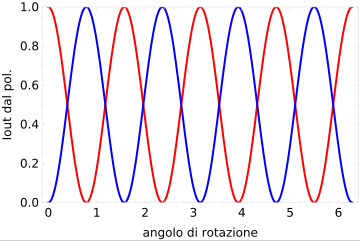
\includegraphics[width=0.6\textwidth]{lambda_mezzi.pdf}
\end{figure} \mbox{} \\
Invece, nella lamina $\frac{\lambda}{4}$, si ha una leggera sovrapposizione dei 
grafici dell'intensità della componente riflessa e trasmessa. 
\begin{figure}[H]
    \centering
    \includesvg[width=0.6\textwidth]{lambda_quarti.svg}
\end{figure} \mbox{} \\
Per quanto riguarda invece il doppio attraversamento, ci si aspetta che le due lamine
$\frac{\lambda}{4}$ e $\frac{\lambda}{2}$ si comportino rispettivamente come delle
lamine $\frac{\lambda}{2}$ e $\lambda$ per un singolo attraversamento.
Tuttavia, per la lamina $\frac{\lambda}{2}$, si osserva come non ci sia una totale
assenza di intensità. Ciò potrebbe essere dovuto da comuni fluttuazioni dei valori del multimetro;
tuttavia è anche possibile che questo sia dovuto da posizionamento o fattura non ideali delle
componenti ottiche costituenti l’apparato sperimentale.
\begin{figure}[H]
    \centering
    \includegraphics[width=0.6\textwidth]{residui-riflessione.pdf}
\end{figure}  \mbox{} \\
Studiando il grafico dei residui (amplificato di un fattore 20) di questa lamina rispetto al fit ideale, si osserva che
i residui (in blu) non seguano l'andamento a 5 picchi del grafico, ma si vadano a
disporre sempre seguendo un andamento sinusoidale formando 3 massimi.
Amplificando per un fattore 20 si è dunque ottenuto il seguente fit:
\begin{figure}[H]
    \centering
    \includegraphics[width=0.55\textwidth]{fit-riflessione.pdf}
\end{figure} \mbox{} \\
Si noti dunque la regolarità dell'andamento dei valori di intensità al
variare dell'angolo per la lamina $\frac{\lambda}{2}$, i quali seguono una sinusoide, seppur
poco pronunciata. Tale andamento è coerente con l'ipotesi di una leggera riflessione
introdotta da errori sistematici dell'apparato sperimentale. 
È possibile, per esempio, che la lamina di ritardo presenti delle imperfezioni che, in
questo caso, sono andate a pesare maggiormente sui residui. Per verificare tale ipotesi
si è provato a simulare un comportamento analogo a quello osservato
per i residui, supponendo che la lamina non sia una lamina $\frac{\lambda}{2}$ perfetta
e che dunque non ritardi la fase di esattamente $\pi$. Si è dunque ottenuto il seguente modello
\begin{figure}[H]
    \centering
    \includegraphics[width=0.55\textwidth]{modello-riflessione.pdf}
\end{figure} \mbox{} \\
Utilizzando un fattore di polarizzazione di $0.2$ sui complessi, il grafico ottenuto
riporta l'andamento di retroriflessione di una lamina con un ritardo di fase di  $\sim 1.18 \pi$.  Riteniamo che, qualitativamente, questo
grafico abbia un andamento comparabile a quello dei residui, per cui si verifica l’ipotesi di lamina di ritardo non ideale. \\
Sulla base delle nostre misure e di queste ultime considerazioni,  possiamo dire sperimentalmente verificate le leggi di Malus.


\end{document}